\chapter{Project Management}
\label{ch:pm}
\section{Risk Management}
Risks were identified in the project specification (\cref{app:spec}). Almost all risks that were met during the project were identified
prior to the project starting. However, the likelihood of some risks was apparently underestimated. For example, the risk of the 
twitter API becoming unavailable was deemed to be very unlikely. This risk was met during the project. Thankfully precautions were
in place to mitigate this risk. The precaution set was to download the tweets in batches and store them locally. Then it would be
possible to create a mock API that would act the same as the real Twitter API. Although this would not work in a commercial setting, it
is valid for realising a prototype as well as setting up unit tests.
\section{Implementation Strategy}
\subsection{Model Creation}
While creating the different models for the topic detection an iterative approach was used. This allowed for the design, implementation and testing
of each model to be done in a short period of time and then move on to the next model. This waterfall-like approach works well for model creation,
especially with the RoBERTa model; the first iteration of the model created the base topic classification model. This model was then used
in the second iteration to create the context aware model.
\begin{figure}[hbtp]
    \centering
    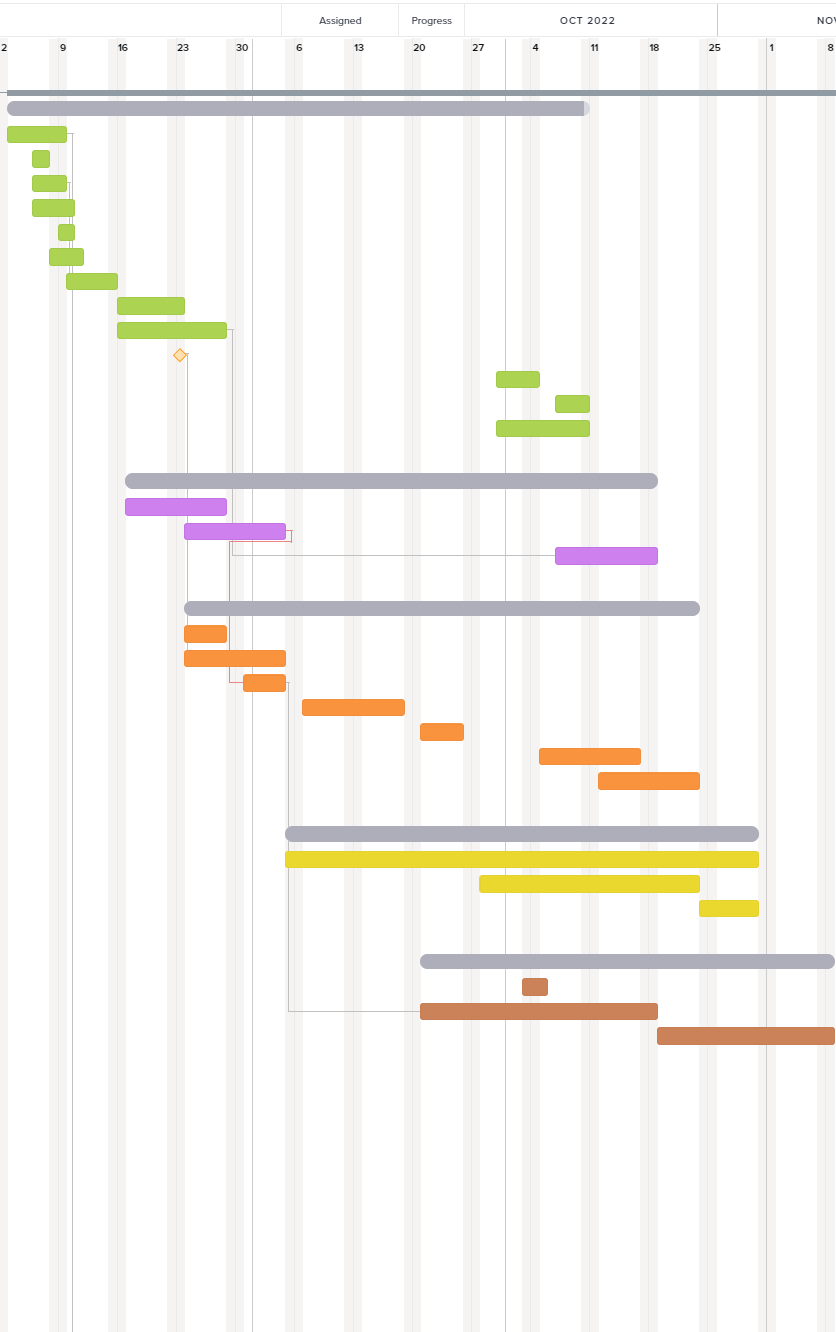
\includegraphics[width=0.5\textwidth]{../images/3yp timeline pres.png}
    \caption{Iterative model creation}
    \label{fig:iterative-model-creation}
\end{figure}

\Cref{fig:iterative-model-creation} shows how the project timeline was split into iterations for the model development. The dashed blue line
shows the separation between the 2 iterations performed in this project.
\subsection{Python Application}
For the Python application, an agile Kanban approach was used. This was partly due to the time constraints, but also because it allowed for
any minor changes required during development to be easily implemented. The Kanban board created consisted of the following columns:
\begin{itemize}
    \item Ideas
    \item Designs
    \item In-Progress
    \item Testing
    \item Completed
\end{itemize}
Due to the fact this project was a solo project, the need for a more complex Kanban board was not required. On top of this, the solo project
means less focus on how items move through the board is required. Usually, items would move using a given protocol (e.g. pull system). For this
project the Kanban board was treated as a simple to-do list and allowed a visual representation of the status of the project.
\begin{figure}[hbtp]
    \centering
    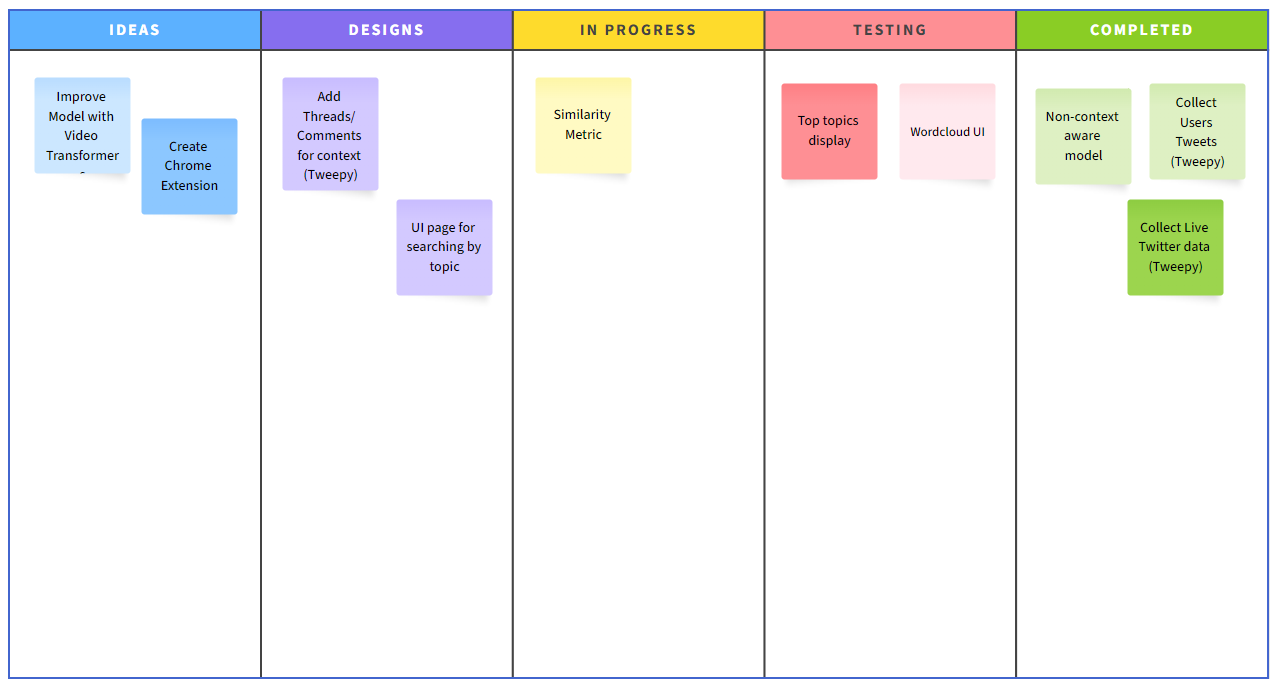
\includegraphics[width=0.8\textwidth]{../images/kanban.png}
    \caption{Kanban board}
    \label{fig:kanban}
\end{figure}

\Cref{fig:kanban} shows the Kanban board (as of 22/02/2023) used during development.

\section{Time Management}
\begin{figure}[hbtp]
    \centering
    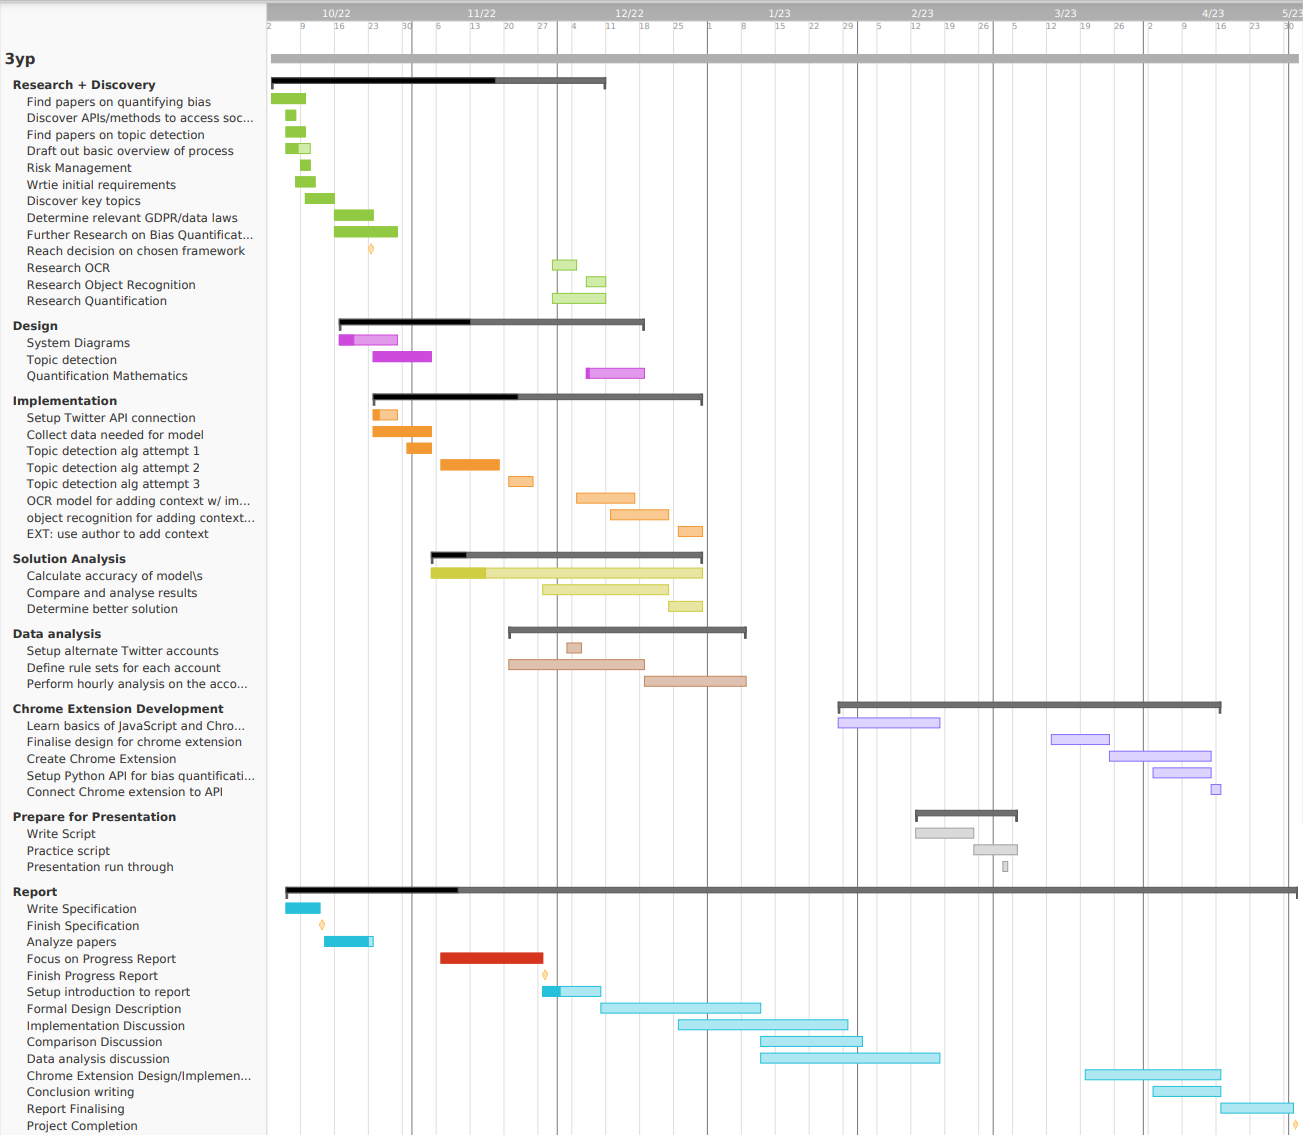
\includegraphics[width=0.8\textwidth]{../images/3yp timeline v3.png}
    \caption{Complete Timetable}
    \label{fig:complete-timetable}
\end{figure}

The method used to set out this timetable was to take the work packages set out in the projects Work Breakdown Structure (WBS)
and assign each work package an amount of time. The idea was to be optimistic with the amount of time required. This is because
it would be a strong motivator to get work done and would give a lot of `slack' time to run into when needed. This was a good
idea because when the progress of this project was halted over christmas due to technical difficulties with DCS batch compute nodes,
there was already the built in slack that meant the project did not fall behind.

\section{Resource Management}
The main resources for this project were:
\begin{itemize}
    \item Application code
    \item Jupyter notebooks for model creation and testing
    \item storage of model parameters for some large models
    \item Training Data for models
\end{itemize}

At the start of the project it was decided Git would be used for version control \cite{git}. This was an easy choice as it is the industry standard
and allows for a structured history of the project to be kept - which we can revert back to if needed. Github was used as the
remote repository for this project. The primary benefits for this were:
\begin{enumerate}
    \item No extra cost
    \item The ability to easily share the code across multiple machines
    \item The ability to create a Continuous Integration (CI) pipeline
\end{enumerate}

There were issues met with the resource management of this project. The main issue was the structure of the repository initially created.
The original plan was to store the code, the reports, and the models in the same repository. Then uses different branches for
updating each of these parts. Although this idea could work, it is far from ideal. It would be best to have a separate repository for
each of these parts. This is something that has been noted during the project and action was taken to rectify this; the report was
separated and moved into it's own repository.

\section{Testing}
\subsection{Model Testing}
Model testing was performed on all models and discussed primarily in \cref{ch:evaluation}. The tests involved calculating the accuracy
of the model on a test set.
\subsection{Unit Testing}
For the application unit testing was performed on the main functions of the application. This was done manually. In retrospect, it would
have been better to use a testing framework such as `Pytest' \cite{pytest}. This would have allowed for a more structured approach to testing and would
make the testing process easier to repeat and report.
\subsection{Integration Testing}
Integration testing was performed to ensure data flowed between the database and UI components correctly. This was done manually.
For example, when ensuring the topic scores were correctly showed on the UI after fetching data from the database, the database
was populated manually and then the UI was checked to ensure the correct data was shown.
\subsection{System Testing}
System testing was performed as a form of acceptance testing. As the main users for this application is the author, the system testing
was performed by the author. This was done by using the application as a user would and ensuring the results were as expected.